\documentclass[10pt]{beamer}

\usetheme[progressbar=frametitle]{metropolis}
\usepackage{appendixnumberbeamer}

\usepackage{booktabs}
\usepackage[scale=2]{ccicons}

\usepackage{pgfplots}
\usepgfplotslibrary{dateplot}

\usepackage{xspace}
\newcommand{\themename}{\textbf{\textsc{metropolis}}\xspace}

% подключаем кириллицу 
\usepackage[T2A]{fontenc}
\usepackage[utf8]{inputenc}
\usepackage{listings}
\usepackage{graphicx}
\usepackage{hyperref}
\usepackage{chronology}


\title{Metropolis}
\subtitle{A modern beamer theme}
% \date{\today}
\date{}
\author{Matthias Vogelgesang}
\institute{Center for modern beamer themes}
% \titlegraphic{\hfill
\includegraphics[height=1.5cm]{logo.pdf}}





\title{Семинар 5}
\subtitle{Введение в С++. Классы.}
%\date{\small{\jobname}}
%\date{\today}
\author{\texttt{Бирюков Владимир}}
\institute{МФТИ}



\begin{document}

%-=-=-=-=-=-=-=-=-=-=-=-=-=-=-=-=-=-=-=-=-=-=-=-=
%
%	TITLE PAGE
%
%-=-=-=-=-=-=-=-=-=-=-=-=-=-=-=-=-=-=-=-=-=-=-=-=

\maketitle


\lstset{language=C}
\defverbatim[colored]\makeset{
\begin{lstlisting}[language=C++,basicstyle=\ttfamily,keywordstyle=\color{blue}]
void make_set(int X) {
  parent[X] = X;
}
\end{lstlisting}
}

\lstset{
  language=C,                % choose the language of the code
  basicstyle=\ttfamily,
  columns=fixed,
  fontadjust=true,
  basewidth=0.5em,
  keywordstyle=\color{blue}\bfseries,
  commentstyle=\color{gray},
  stringstyle=\ttfamily\color{yellow!40!red},
  showstringspaces=false,
  %numbers=false,                   % where to put the line-numbers
  numbersep=5pt,
  numberstyle=\tiny\color{gray},
  numberfirstline=true,
  stepnumber=1,                   % the step between two line-numbers.        
  numbersep=5pt,                  % how far the line-numbers are from the code
  backgroundcolor=\color{white!90!gray},  % choose the background color. You must add \usepackage{color}
  showstringspaces=false,         % underline spaces within strings
  captionpos=b,                   % sets the caption-position to bottom
  breaklines=true,                % sets automatic line breaking
  breakatwhitespace=true,         % sets if automatic breaks should only happen at whitespace
}
\lstset{literate=%
   *{0}{{{\color{red!20!violet}0}}}1
    {1}{{{\color{red!20!violet}1}}}1
    {2}{{{\color{red!20!violet}2}}}1
    {3}{{{\color{red!20!violet}3}}}1
    {4}{{{\color{red!20!violet}4}}}1
    {5}{{{\color{red!20!violet}5}}}1
    {6}{{{\color{red!20!violet}6}}}1
    {7}{{{\color{red!20!violet}7}}}1
    {8}{{{\color{red!20!violet}8}}}1
    {9}{{{\color{red!20!violet}9}}}1
}
%\begin{frame}[plain]
%	\titlepage
%\end{frame}

%-=-=-=-=-=-=-=-=-=-=-=-=-=-=-=-=-=-=-=-=-=-=-=-=
%
%	TABLE OF CONTENTS: OVERVIEW
%
%-=-=-=-=-=-=-=-=-=-=-=-=-=-=-=-=-=-=-=-=-=-=-=-=

\section{ООП. Классы}

\begin{frame}[fragile]
\frametitle{Программирование} 
\begin{center}
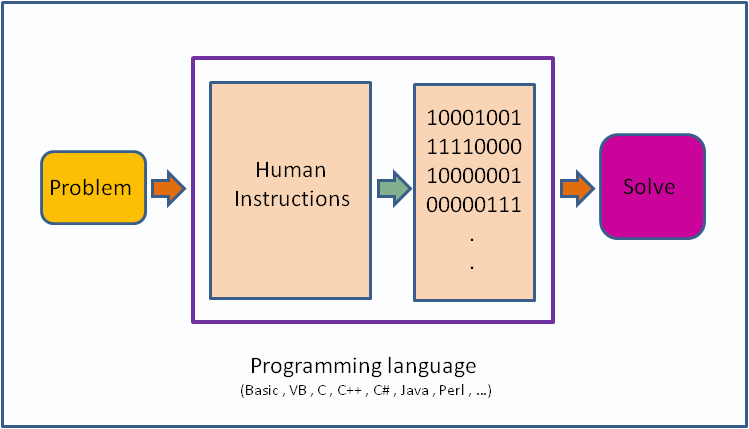
\includegraphics[width=0.65\linewidth]{images/programming.png}
\end{center}
\textbf{Парадигмы программирования:}
\begin{itemize}
\item \textbf{Процедурное} -- отражение архитектуры традиционных ЭВМ.\\
C, Pascal, C++, python
\item \textbf{Объектно-ориентированное} -- представление программы в виде совокупности объектов.
Java, C\#, C++, python
\item \textbf{Функциональное} -- процесс вычисления как вычисление некой математической функции. Haskell
\end{itemize}
\end{frame}

\begin{frame}[fragile]
\frametitle{ООП} 
\textbf{ООП} — методология программирования, основанная на представлении программы в виде совокупности объектов, каждый из которых является экземпляром определенного класса, а классы образуют иерархию наследования. \\
\textbf{Основные принципы:}
\begin{itemize}
\item Инкапсуляция
\item Наследование
\item Полиморфизм
\end{itemize}
\end{frame}

\begin{frame}[fragile]
\frametitle{ООП в стиле C} 
\begin{lstlisting}[language=C++,basicstyle=\ttfamily,keywordstyle=\color{blue}]
struct Monster
{
    float x, y, z;
    int health, is_alive, power;
};

void hurt_monster(Monster* m, int damage)
{
    m->health -= damage;
    if (m->health < 0)
        m->is_alive = 0;
}
void heal_monster(Monster* m, int heal_power)
{
    m->health += heal_power;
}
\end{lstlisting}
\end{frame}

\begin{frame}[fragile]
\frametitle{ООП в стиле C++} 
\begin{lstlisting}[language=C++,basicstyle=\ttfamily,keywordstyle=\color{blue}]
struct Monster
{
    float x, y, z;
    int health, is_alive, power;
    
    void hurt(int damage)
    {
        m->health -= damage;
        if (m->health < 0)
            m->is_alive = 0;
    }
    void heal(int heal_power)
    {
        m->health += heal_power;
    }
};
\end{lstlisting}
\end{frame}

\begin{frame}[fragile]
\frametitle{Инкапсуляция} 
\begin{lstlisting}[language=C++,basicstyle=\ttfamily,keywordstyle=\color{blue}]
class Monster
{
private:
    float x, y, z;
    int health, is_alive, power;
public:
    void hurt(int damage)
    {
        m->health -= damage;
        if (m->health < 0)
            m->is_alive = 0;
    }
    void heal(int heal_power)
    {
        m->health += heal_power;
    }
};
\end{lstlisting}
\end{frame}


\begin{frame}[fragile]
\frametitle{ООП в стиле C++} 
\begin{lstlisting}[language=C++,basicstyle=\ttfamily,keywordstyle=\color{blue}]
struct Monster
{
    float x, y, z;
    int health, is_alive, power;
    void hurt(int damage);
    void heal(int heal_power);
};
void Monster::hurt(int damage)
{
    m->health -= damage;
    if (m->health < 0)
        m->is_alive = 0;
}
void Monster::heal(int heal_power)
{
    m->health += heal_power;
}
\end{lstlisting}
\end{frame}

\section{Ввод вывод в C++. iostream}

\begin{frame}[fragile]
\frametitle{iostream} 
\begin{lstlisting}[language=C++,basicstyle=\ttfamily,keywordstyle=\color{blue}]
#include <iostream>

int main 
{
    std::cout << "Hello world! " << 42 << std::endl;    
    int a;
    std::cin >> a;
}
\end{lstlisting}
\end{frame}

\begin{frame}[fragile]
\frametitle{iostream} 
\begin{lstlisting}[language=C++,basicstyle=\ttfamily,keywordstyle=\color{blue}]
#include <iostream>
using namespace std;

int main 
{
    cout << "Hello world! " << 42 << endl;    
    int a;
    cin >> a;
}
\end{lstlisting}
\end{frame}


\section{Раздельная компиляция}

\begin{frame}[fragile]
\frametitle{Компилируемый язык} 
Язык C является компилируемым языком программирования \\
Компиляция -- преобразование текста программы(исходного кода) в машинный код. \\
\quad\\
Зачем разбивать программу на файлы?
\begin{enumerate}
\item С небольшими файлами удобнее работать
\item Ускорения повторной компиляции при небольших изменениях
\item Структуирование кода
\end{enumerate}
\end{frame}

\begin{frame}[fragile]
\frametitle{Общая схема сборки программы} 
\begin{center}
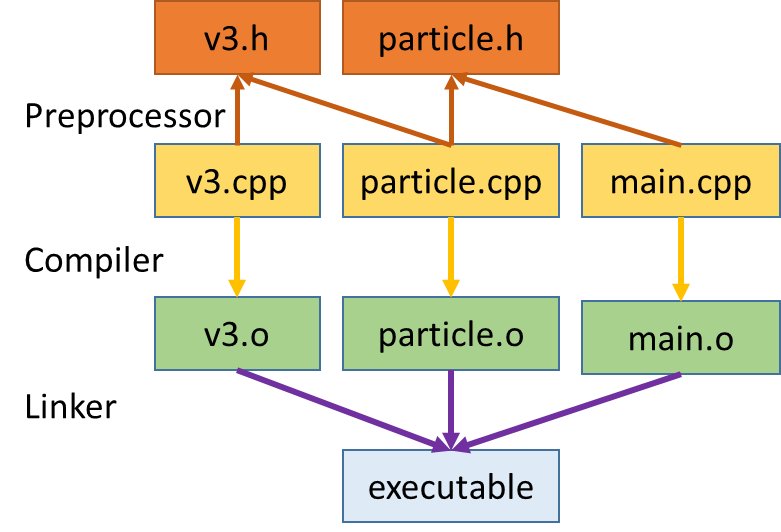
\includegraphics[width=0.95\linewidth]{images/separate_compilation_linking.png}
\end{center}
\end{frame}





\end{document}